% =========================================================================
% CAPITOLO 4 — INQUADRAMENTO SCIENTIFICO
% =========================================================================

\chapter{Inquadramento scientifico}
\label{ch:background}

\noindent
{\rmfamily\itshape
\begin{tabular}[t]{@{}l@{\hspace{0.3cm}}p{12.5cm}@{}}
\textls[50]{\textbf{Trattati:}} &
\textls[50]{Sistema fisico · Circolazione termoalina · Bistabilità e tipping · Isteresi ·
Misura e unità · Dati osservativi e rianalisi}
\end{tabular}
}

\vspace{0.5cm}

Questo capitolo spiega che cos'è l'AMOC: come funziona come sistema fisico, perché può passare da uno stato all'altro, come se ne misura l'intensità e quali record esistono. È volutamente breve. Qui è incluso solo ciò che i capitoli successivi usano effettivamente --- ciò che la fase di \emph{rilevamento} scompone e ciò che la fase di \emph{traduzione} deve rendere percepibile.

% -------------------------------------------------------------------------
\section{Il sistema fisico}
\label{sec:bg-physical}

La Atlantic Meridional Overturning Circulation è il nastro trasportatore di calore dell'oceano attraverso l'Atlantico. L'acqua superficiale calda e salata scorre verso nord; nei freddi mari subpolari cede calore all'atmosfera, diventa densa e sprofonda; torna quindi verso sud in profondità come corrente fredda e profonda (Figura~\ref{fig:amoc-schematic}). Questo rovesciamento verticale --- flusso superficiale in un verso, flusso profondo nell'altro --- è guidato da differenze di densità dell'acqua determinate da temperatura e salinità, il processo noto come circolazione termoalina.

% it/figures/background/amoc_schematic.tex — versione italiana
\begin{figure}[!ht]
    \centering
    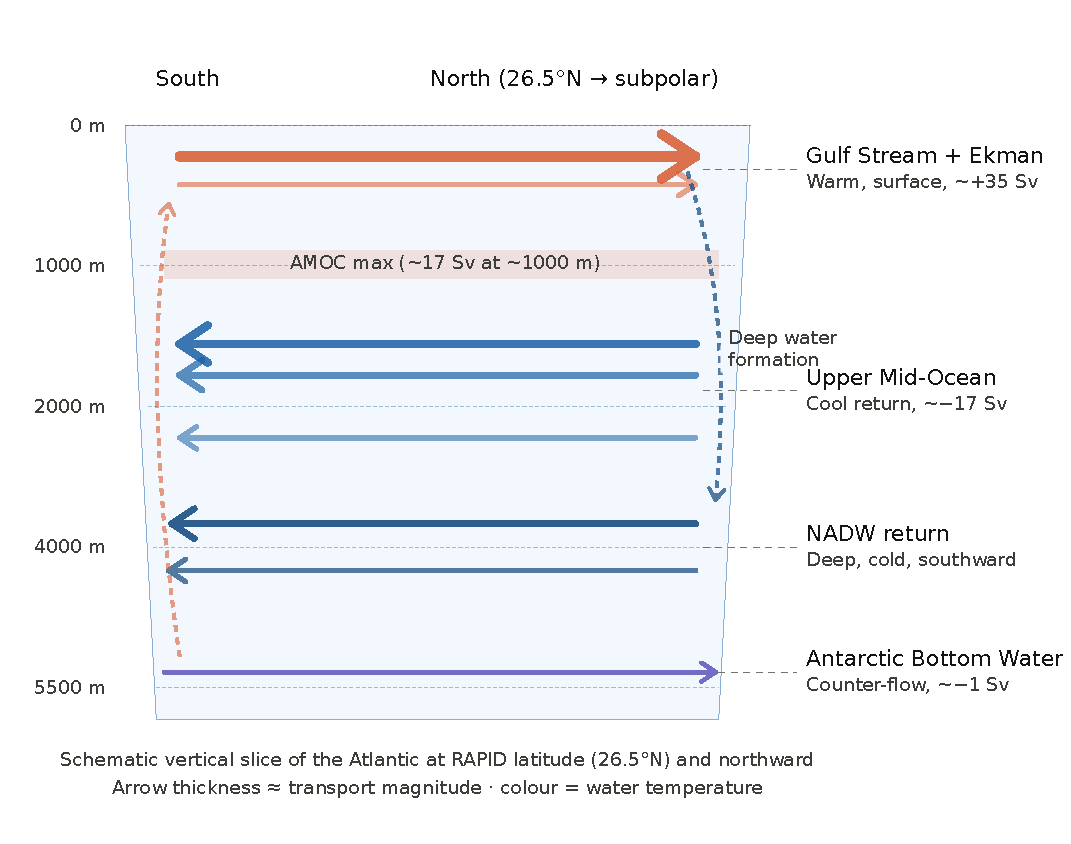
\includegraphics[width=0.9\textwidth]{figures/background/amoc_atlantic_cross_section.pdf}
    \caption[La circolazione di rovesciamento atlantica.]{\textbf{La circolazione di
    rovesciamento atlantica in sezione trasversale.} L'acqua calda superficiale fluisce
    verso nord (arancione), cede calore all'atmosfera nei mari subpolari, diventa densa
    e sprofonda, e ritorna verso sud come una fredda corrente profonda (blu). Il
    rovesciamento verticale è guidato dalle differenze di densità dovute a temperatura
    e salinità. La circolazione non ha alcuna espressione visibile in superficie ---
    l'invisibilità che la tesi si propone di affrontare.}
    \label{fig:amoc-schematic}
\end{figure}


La conseguenza è climatica, non meramente oceanografica. Il flusso superficiale verso nord trasporta nel Nord Atlantico dell'ordine di un petawatt di calore --- paragonabile alla produzione di un milione di grandi centrali elettriche --- e gran parte della relativa mitezza dell'Europa nord-occidentale dipende da esso \citep{buckley2016}. Eppure il sistema non ha alcuna superficie che un osservatore possa vedere: è una circolazione nell'interno dell'oceano, estesa su un bacino, che si dispiega su decenni. È proprio questo il divario che la tesi affronta --- un processo di grande portata e di nessuna visibilità quotidiana.

% -------------------------------------------------------------------------
\section{Bistabilità e tipping}
\label{sec:bg-bistability}

Ciò che rende l'AMOC un \emph{elemento di tipping}, anziché un sistema che semplicemente si indebolisce in proporzione al riscaldamento, è un meccanismo di retroazione colto per la prima volta da \citet{stommel1961} in un semplice modello dell'oceano a due scatole.\footnote{Stommel rappresentò l'oceano come due scatole, equatoriale e polare, che si scambiano acqua a un tasso fissato dalla loro differenza di densità. La retroazione di avvezione del sale nelle sue equazioni produce due equilibri stabili per lo stesso forzante esterno --- la firma matematica della bistabilità.} Il meccanismo è un ciclo: il rovesciamento trasporta sale verso nord, il sale mantiene densa l'acqua settentrionale, e l'acqua densa continua a sprofondare, sostenendo il rovesciamento. Si aggiunga abbastanza acqua dolce al Nord Atlantico --- dal ghiaccio che si scioglie, per esempio --- e il ciclo può girare al contrario: acqua più dolce è meno densa, lo sprofondamento si indebolisce, meno sale viene portato a nord, e la circolazione si rallenta ulteriormente da sé.

A causa di questa retroazione, l'AMOC ha due stati stabili --- un rovesciamento vigoroso e uno molto più debole --- per le stesse condizioni. Una spinta graduale può quindi innescare un passaggio brusco, e invertire la spinta non inverte semplicemente il passaggio.

Questa proprietà, chiamata isteresi, è la ragione per cui il comportamento del sistema è non lineare e per cui resiste all'intuizione: causa ed effetto non sono proporzionali. Comunicare quella non linearità, che nessuna curva statica trasmette, è la sfida di rappresentazione al centro di questa tesi.

% -------------------------------------------------------------------------
\section{Misurare la circolazione}
\label{sec:bg-measurement}

Per analizzare l'AMOC, la sua intensità va espressa come numero. Quel numero è il volume d'acqua che il rovesciamento muove, misurato in \emph{sverdrup} (\SI{1}{\sverdrup} = \SI{e6}{\cubic\metre\per\second} --- un milione di metri cubi al secondo).\footnote{Formalmente, la funzione di corrente del rovesciamento integra la velocità verso nord attraverso il bacino e verso il basso dalla superficie; il suo massimo lungo la profondità definisce il trasporto AMOC a una data latitudine.} Un tipico rovesciamento alle medie latitudini si attesta su circa \SIrange{15}{20}{\sverdrup}.

Cosa cruciale per ciò che segue, la circolazione non è un singolo numero ma un \emph{profilo}: il trasporto varia con la profondità, forte vicino alla superficie dove l'acqua calda scorre verso nord, invertendosi in profondità dove l'acqua fredda torna verso sud. Questo profilo verticale, risolto nel tempo, è la materia prima che la fase di \emph{rilevamento} scompone --- l'oggetto da cui il machine learning recupera una struttura latente compatta nel Capitolo~\ref{ch:data_pipeline}.

% -------------------------------------------------------------------------
\section{Dati osservativi}
\label{sec:bg-data}

L'AMOC è osservata direttamente dall'array RAPID-MOCHA-WBTS (Rapid Climate Change --- Meridional Overturning Circulation and Heatflux Array --- Western Boundary Time Series) a \ang{26.5}~nord, una linea di strumenti ormeggiati che attraversa l'Atlantico e che misura il rovesciamento con continuità dal 2004 \citep{frajkawilliams2021, moat2026}. RAPID è l'àncora empirica di questa tesi: un record autentico e continuo di un sistema che in precedenza era stato solo dedotto.

Il suo unico limite è la lunghezza. Due decenni di dati sono pochi rispetto a una circolazione che varia su scale da decenni a secoli, perciò il record osservato non può da solo rivelare il comportamento lento del sistema. Per fornire un contesto più lungo, l'analisi aggiunge l'ensemble Copernicus Marine GREP --- una rianalisi che ricostruisce la circolazione prima del periodo osservativo combinando modelli con dati assimilati, al prezzo di introdurre una dipendenza dai modelli e una dispersione tra i membri dell'ensemble. Quella dispersione non è una mera avvertenza: diventa, nella fase di \emph{traduzione}, la forma grezza di incertezza che la rappresentazione deve rendere percepibile. Insieme, osservazione e rianalisi sono i due insiemi di dati che il capitolo successivo analizza.
